\documentclass[tikz]{standalone}
\usepackage{graphicx} % Required for inserting images
\usepackage{tikz}
\usepackage{amsmath}
\usepackage{xcolor}
\usetikzlibrary{shadows}
\usetikzlibrary{backgrounds}
\usetikzlibrary{patterns.meta}
\usetikzlibrary{patterns}
\usetikzlibrary {arrows.meta,automata,positioning,fit,calc,matrix,math}

\definecolor{process_step_background}{HTML}{FFFAF0}
\definecolor{intermediate_fill_colour}{HTML}{949698}

\tikzset{
diagonal fill/.style 2 args={fill=#2, path picture={
\fill[#1, sharp corners] (path picture bounding box.south west) -|
                         (path picture bounding box.north east) -- cycle;}},
reversed diagonal fill/.style 2 args={fill=#2, path picture={
\fill[#1, sharp corners] (path picture bounding box.north west) |- 
                         (path picture bounding box.south east) -- cycle;}}
}

\tikzstyle{InputAndOutputState} =[diagonal fill={red}{green},rounded corners,draw]
 
\tikzstyle{process_step_node} =[fill=process_step_background,rounded corners]
\tikzstyle{intermediate_state} = [fill=intermediate_fill_colour,rounded corners,state,rectangle]

\begin{document}
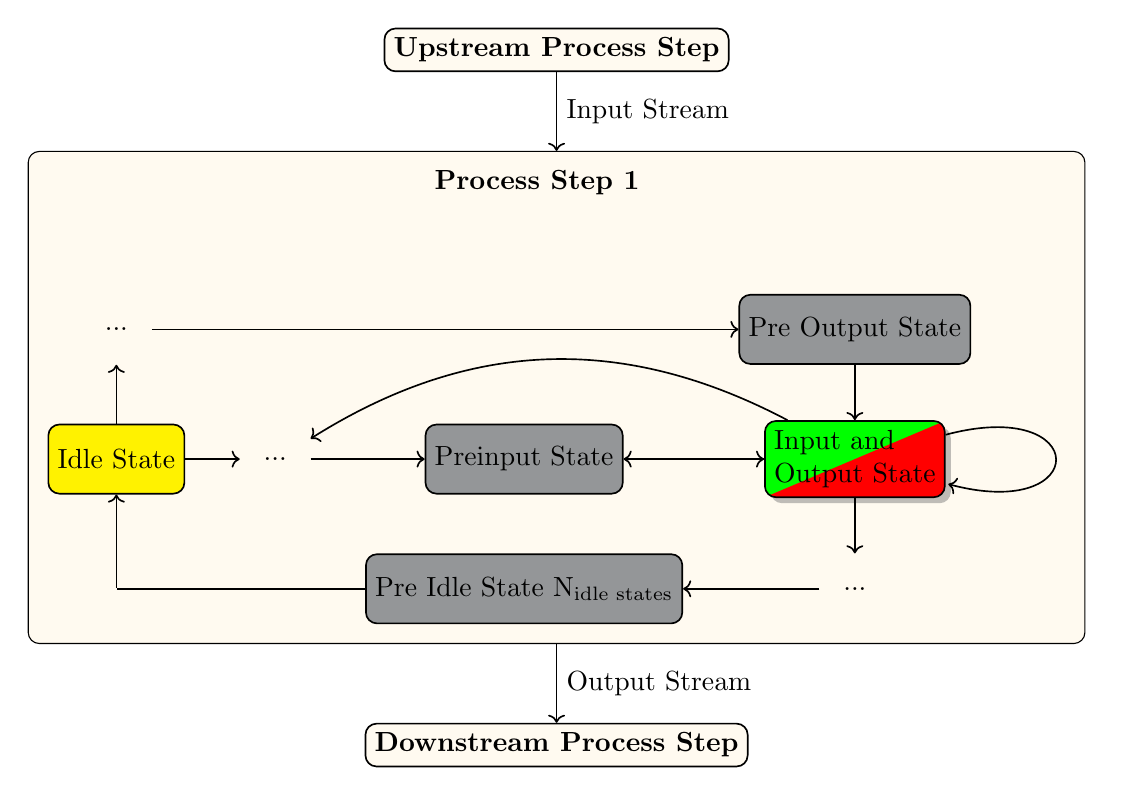
\begin{tikzpicture}[->,auto,node distance=1cm,on grid,semithick]



    \matrix [column sep=20,row sep=20](process_step_matrix)
    {


        \node[state,rounded corners,rectangle,draw=none](direct_output_at_idle_column){...};                         &
        \node[state,rounded corners,rectangle,draw=none]{};                                                          &
        \node[state,rounded corners,rectangle,draw=none]{};                                                          &
        \node[intermediate_state](direct_pre_output_state){Pre Output State};                                        & \\



        \node[state,rounded corners,rectangle,style={fill=yellow}](idle_process_state){Idle State};       &
        \node[state,rounded corners,rectangle,draw=none](output_statebetween_idle_and_input_and_output){...};        &
        \node[intermediate_state](pre_input_and_output_stream_state){Preinput State};                                &
        \node[InputAndOutputState,align=left, drop shadow](input_and_output_stream_state){Input and\\ Output State}; & \\

        \node[state,rounded corners,circle,draw=none,inner sep=0pt,minimum size=0pt](first_idle_connection_node){};  &
        \node[state,rounded corners,rectangle,draw=none]{};                                                          &
        \node[intermediate_state](pre_idle_state){Pre Idle State {$\text{N}_\text{idle states}$}};                           &
        \node[state,rounded corners,rectangle,draw=none](between_output_and_preidle_state){...};                       \\
    };



    % Direct Idle to Output connections
    \draw (idle_process_state) to (direct_output_at_idle_column);
    \draw (direct_output_at_idle_column) to (direct_pre_output_state);
    \draw (direct_pre_output_state) to (input_and_output_stream_state);

    % Input recycle
    \path (input_and_output_stream_state) edge [loop right] node (self_loop_node){} (input_and_output_stream_state);
    \draw (input_and_output_stream_state) to (pre_input_and_output_stream_state);
    \draw (input_and_output_stream_state) to [bend right](output_statebetween_idle_and_input_and_output);



    % Idle to Output over input state
    \draw (idle_process_state) to (output_statebetween_idle_and_input_and_output);
    \draw (output_statebetween_idle_and_input_and_output) to (pre_input_and_output_stream_state);
    \draw (pre_input_and_output_stream_state) to (input_and_output_stream_state);


    % %Output to idle
    \draw (input_and_output_stream_state) to (between_output_and_preidle_state);
    \draw (between_output_and_preidle_state) to (pre_idle_state);
    \draw[-] (pre_idle_state) to (first_idle_connection_node);
    \draw (first_idle_connection_node) to (idle_process_state);




    % Frame and label for process step
    \node[above= of process_step_matrix.north] (test)  {\textbf{Process Step 1}};
    \begin{scope}[on background layer]
        \node[draw,fit=(test)(process_step_matrix)(self_loop_node),process_step_node](process_step_outer_frame){};
    \end{scope}
    % Upstream and downstream nodes and connections    
    \node[draw,above= of process_step_outer_frame.north,process_step_node] (upstream_process_step){\textbf{Upstream Process Step}};
    \node[draw,below= of process_step_outer_frame.south,process_step_node] (downstream_process_step){\textbf{Downstream Process Step}};
    \draw (upstream_process_step) ->  (process_step_outer_frame) node[midway]{Input Stream};
    \draw (process_step_outer_frame) -> (downstream_process_step) node[midway]{Output Stream};







\end{tikzpicture}
\end{document}
